\chapter{Architecture Design}
\label{chap:architecture_design}

\section*{Introduction}
This chapter provides a detailed exploration of the system architecture, which is designed to be modular, scalable, and secure. Key components include the integration of Large Language Models (LLMs), the implementation of a highly specialized Retrieval-Augmented Generation (RAG) architecture, modern frontend and backend frameworks, and supporting services such as vector databases and logging telemetry. Each architectural component is designed to interact seamlessly while ensuring optimal performance, strict tenant isolation, and high robustness.

\pagebreak

\section{Detailed Component Architecture}

The platform's backend architecture follows a highly decoupled approach using FastAPI. This ensures that services are modular, asynchronous, and scalable.

\subsection{Data Management}
The backend efficiently manages relational data storage and retrieval using PostgreSQL via the \texttt{asyncpg} driver and SQLAlchemy, ensuring high responsiveness even under heavy concurrent loads. 
To guarantee strict tenant isolation, user-uploaded files and generated \LaTeX\ projects are stored in dedicated directories on the server. Access is strictly mediated by Row-Level Security (RLS) policies and Foreign Keys tied to the authenticated user's unique ID. A user must be fully authenticated to gain access to their personal vault; no files are publicly exposed.

\subsection{System Logging \& Telemetry}
To maintain enterprise-grade observability, we engineered a custom, asynchronous Logging System that acts as the central nervous system of the backend.
\begin{itemize}
    \item \textbf{Purpose:} The logging system tracks every incoming HTTP request, database query latency, unhandled exceptions, and RAG pipeline operations (chunking, embedding, retrieval). It allows administrators to trace errors and monitor the performance of the AI models in real-time.
    \item \textbf{Mechanism:} Logs are formatted as structured JSON for machine-readability. To preserve disk space, the system uses a \texttt{TimedRotatingFileHandler}. Every night at midnight, the active log file is rotated, compressed into a \texttt{.gz} archive, and stored in the \texttt{/logs} directory. The system autonomously retains 30 days of history, automatically deleting archives older than a month to prevent storage overflow. Sensitive data (such as API keys and JWTs) are scrubbed via Regex before being written to disk.
\end{itemize}

\IfFileExists{Figures/log_architecture.png}{
    \begin{figure}[H]
        \centering
        \includegraphics[width=0.8\textwidth]{Figures/log_architecture.png}
        \caption{Architecture of the Rotating JSON Log System}
        \label{fig:log_system}
    \end{figure}
}{}

\subsection{Authentication \& APIs}
\textbf{Authentication:} We integrated \textbf{Clerk} for Identity and Access Management (IAM). Clerk handles multi-provider authentication (OAuth) and generates secure JSON Web Tokens (JWTs). The FastAPI backend intercepts every request using a custom dependency that decodes the JWT, verifies its signature against Clerk's dynamic JSON Web Key Set (JWKS), and extracts the user ID to enforce data ownership.

\textbf{APIs:} The API is fully asynchronous and documented automatically via Swagger UI. It acts as the orchestration layer, managing internal routes for the Chat Interface, Document Management System (DMS), and communicating with external APIs (Google Gemini, OpenAI, and LaTeXLite).

\IfFileExists{Figures/backend_architecture.png}{
    \begin{figure}[H]
        \centering
        \includegraphics[width=0.9\textwidth]{Figures/backend_architecture.png}
        \caption{Detailed Backend Component Architecture}
        \label{fig:backend_arch}
    \end{figure}
}{}

\newpage
\section{RAG Architecture \& Intelligence Pipeline}

Our Retrieval-Augmented Generation (RAG) architecture diverges from standard implementations to specifically handle the morphological complexities of Moroccan legal documents in Arabic.

\subsection{The Offline Ingestion Pipeline}
Instead of relying on generic open-source OCR (Optical Character Recognition) libraries, which struggle with scanned Arabic matrices and legal stamps, we utilize a Vision-Language Model (\textbf{GPT-4o Vision}). The PDF is converted into images and sent to the model alongside a highly engineered, domain-specific prompt.

This prompt strictly enforces noise filtering (ignoring headers, footers, and stamps) and forces the LLM to output semantic XML tags (\texttt{<chunk>} and \texttt{<table>}). A snippet of this critical System Prompt is detailed below:

\begin{quote}
\textit{"أنت خبير متقدم ومحلف في هندسة البيانات وتحليل النصوص من الوثائق الإدارية والقانونية... يجب ألا تدخل المعلومات التالية في قاعدة البيانات لأنها تكرار يفسد البحث: تجاهل الترويسة العلوية المتكررة: المملكة المغربية، وزارة الاقتصاد والمالية... استخرج النص كما هو بالضبط. لا تلخص، ولا تشرح... You MUST extract tables in Markdown format and wrap them exactly like this: <table> <title> Write a highly descriptive Arabic title... </title> <content> ... </content> </table>"}
\end{quote}

Once extracted, our custom Python parser splits the XML tags. For text chunks, the entire block is embedded using \texttt{BAAI/bge-m3} and saved to \textbf{ChromaDB}. For tables, a critical optimization is applied: only the descriptive \texttt{<title>} is embedded mathematically, while the full Markdown \texttt{<content>} is preserved as metadata payload.

\subsection{Retrieval \& Generation}
When a user asks a question, the backend embeds the query and performs a cosine similarity search on ChromaDB to retrieve the Top 20 chunks. These chunks are then passed through a Cross-Encoder (\texttt{BAAI/bge-reranker}) to isolate the Top 5 most semantically relevant results. Finally, these 5 chunks are assembled into an augmented prompt and sent to \textbf{Google Gemini 2.5 Flash} to generate the final, highly accurate response.

\IfFileExists{Figures/seq_rag_pipeline.png}{
    \begin{figure}[H]
        \centering
        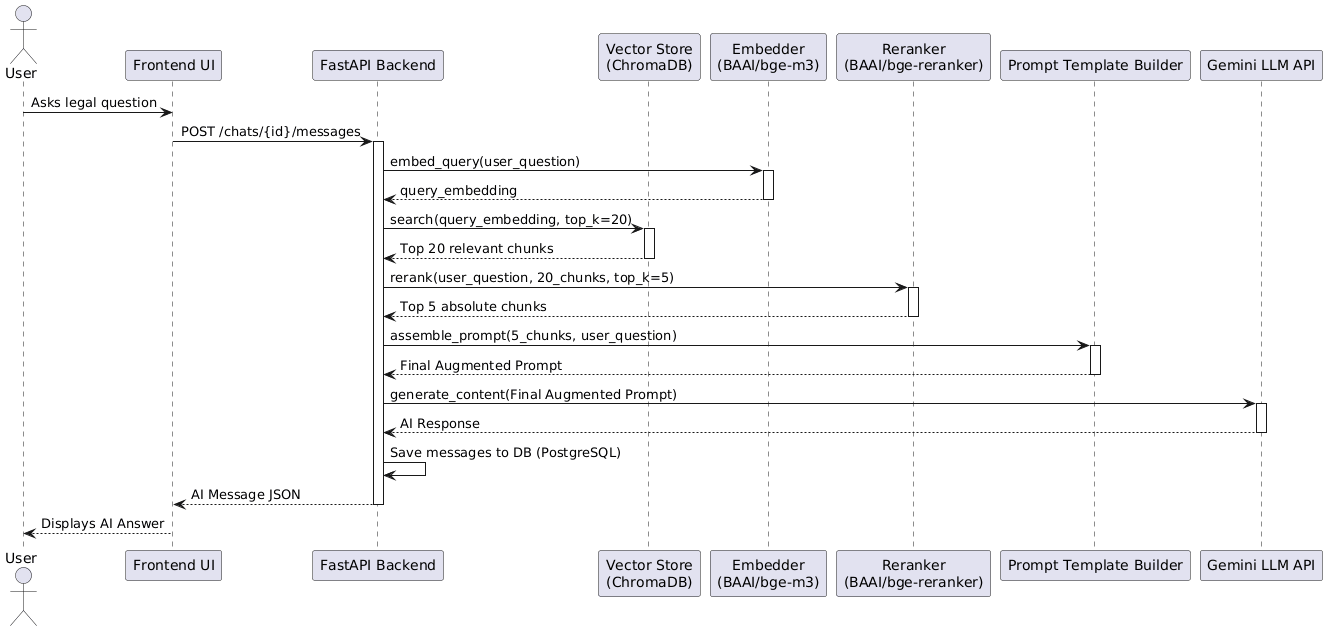
\includegraphics[width=0.9\textwidth]{Figures/seq_rag_pipeline.png}
        \caption{RAG Pipeline Execution Architecture}
        \label{fig:rag_arch}
    \end{figure}
}{}

\newpage
\section{Frontend Design \& User Experience}

The frontend is a Single Page Application (SPA) built with \textbf{React 19} and \textbf{Vite}. It employs a modular component architecture and a clean, enterprise-grade dark/light user interface inspired by modern platforms like Notion.

\subsection{Application Routing Tree}
The application leverages \texttt{react-router-dom} to manage client-side navigation seamlessly without reloading the browser. The route structure is organized as follows:

\begin{verbatim}
/ (Root)
|-- /sign-in                  -> Authentication Portal (Clerk)
|-- /sign-up                  -> Registration Portal (Clerk)
|-- /                         -> Landing Page (Public overview & features)
|
|-- /chat                     -> Main AI Interface
|   |-- /chat/:id             -> Specific AI Conversation Thread
|
|-- /database                 -> Document Management System (DMS)
|                                (Virtual folders, upload, pagination, sorting)
|
|-- /editor                   -> Workspace for LaTeX Generation
|   |-- /editor/:id           -> Split-Screen Editor (Code / PDF Viewer / AI)
|
|-- /lawyers                  -> Professional Directory & Messaging
\end{verbatim}

\subsection{UI Optimization}
The frontend implements specialized rendering layers. For instance, the Chat Page utilizes \texttt{react-markdown} combined with custom CSS logic (\texttt{unicode-bidi: plaintext}) to autonomously detect and perfectly align Arabic text Right-To-Left (RTL), while keeping French/English terminology Left-To-Right (LTR) within the same paragraph. State management is handled through React Hooks, ensuring that operations like inline renaming of folders or live file uploads are instantaneous and reactive.

\IfFileExists{Figures/use_case.png}{
    \begin{figure}[H]
        \centering
        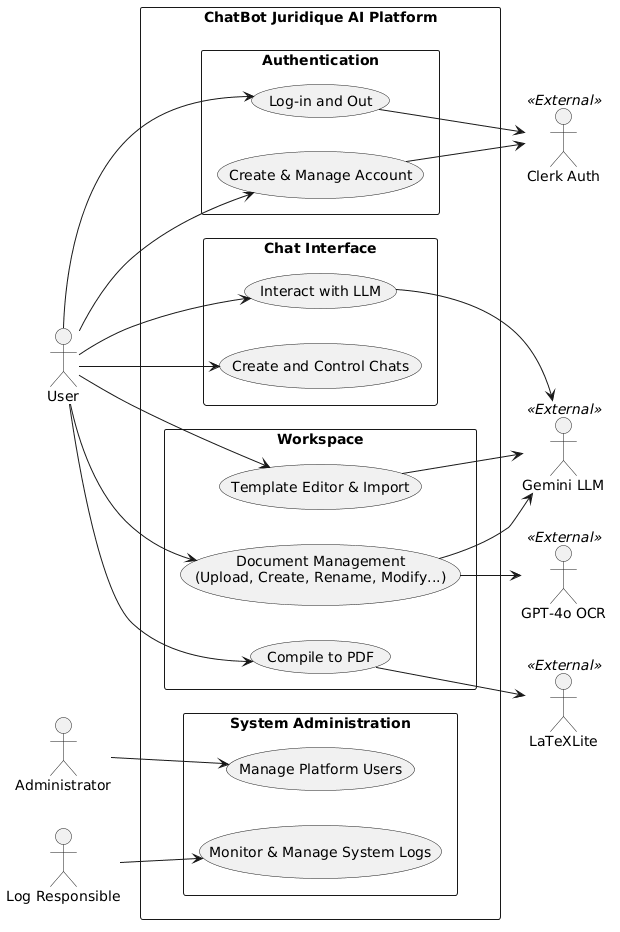
\includegraphics[width=0.8\textwidth]{Figures/use_case.png}
        \caption{Platform Use Case Diagram}
        \label{fig:frontend_usecase}
    \end{figure}
}{}

\newpage
\section*{Conclusion}
The architecture designed for this platform successfully bridges the gap between complex legal data processing and seamless user interaction. By decoupling the heavy RAG ingestion pipeline from the main web server, implementing a robust custom logging system, and utilizing an asynchronous FastAPI backend paired with a reactive React frontend, the system achieves enterprise-grade stability and performance.
